\documentclass[11pt]{article}
\usepackage[a4paper,margin=2.5cm]{geometry}
\usepackage{amsmath,amssymb,amsthm,mathtools}
\usepackage{newpxtext,newpxmath}
\usepackage[scaled=0.92]{sourcesanspro}
\usepackage{microtype}
\usepackage{graphicx}
\usepackage{booktabs,tabularx}
\usepackage{enumitem}
\usepackage[dvipsnames]{xcolor}
\usepackage[most]{tcolorbox}
\usepackage{titlesec}
\usepackage{caption}
\usepackage[hyphens]{url}
\usepackage{hyperref}

\definecolor{navy}{HTML}{1F3A5F}
\definecolor{accent}{HTML}{D9822B}
\definecolor{warn}{HTML}{B23A48}
\hypersetup{colorlinks,linkcolor=navy,citecolor=navy,urlcolor=navy}
\captionsetup{font=small,labelfont={bf,color=navy}}
\titleformat{\section}{\sffamily\Large\bfseries\color{navy}}{\thesection}{0.8em}{}
\titleformat{\subsection}{\sffamily\large\bfseries\color{navy}}{\thesubsection}{0.8em}{}
\setlist{itemsep=2pt,topsep=4pt}
\emergencystretch=2em

\newtheorem{theorem}{Theorem}
\newtheorem{corollary}{Corollary}[section]
\newtheorem{proposition}[corollary]{Proposition}
\theoremstyle{remark}
\newtheorem{remark}[corollary]{Remark}
\newtheorem{example}[corollary]{Example}

\newcommand{\R}{\mathbb{R}}
\newcommand{\N}{\mathbb{N}}
\newcommand{\ip}[2]{\langle #1,#2\rangle}
\newcommand{\BC}{\mathrm{BC}}
\DeclareMathOperator{\Gram}{Gram}

\newtcolorbox{keybox}[1][]{enhanced,colback=navy!4,colframe=navy!60,boxrule=0.6pt,arc=2pt,left=8pt,right=8pt,top=6pt,bottom=6pt,fonttitle=\sffamily\bfseries,coltitle=navy,colbacktitle=navy!10,#1}
\newcommand{\claimtag}[2]{\tcbox[on line,boxsep=1pt,left=3pt,right=3pt,top=0pt,bottom=0pt,colback=#1!10,colframe=#1!70,boxrule=0.4pt,arc=1.5pt]{\sffamily\scriptsize\bfseries\color{#1}#2}}
\newcommand{\context}{\claimtag{navy}{CONTEXT}}
\newcommand{\consequence}{\claimtag{ForestGreen}{PROVED HERE}}
\newcommand{\proposal}{\claimtag{accent}{PROPOSAL}}
\newcommand{\nofollow}{\claimtag{warn}{DOES NOT FOLLOW}}

\begin{document}

\begin{center}
{\sffamily\small\color{navy} APPLICATIONS REPORT \quad\textbullet\quad PRINCIPIA MATH, MATHDB 369283}\\[10pt]
{\sffamily\LARGE\bfseries\color{navy} What a Cauchy--Schwarz inequality\\[2pt] for real powers is good for}\\[8pt]
{\large Consequences in matrix analysis, probability, statistical physics,\\ machine learning and quantum information}\\[12pt]
Pragyaan Gaur \quad\textbullet\quad 8 October 2026
\end{center}

\begin{keybox}[title=Summary]
For nonnegative vectors $v,w$ and a real number $p\ge2$,
\[
\|v^p\|\,\|w^p\|-\ip{v^p}{w^p}\;\le\;\|v\|^p\|w\|^p-\ip vw^p,
\]
where $v^p$ is the vector of $p$-th powers of the entries. This was Conjecture~5.1 of Johnston, Plosker, Torrance and Varona~\cite{JPTV}, and it is proved in the accompanying paper~\cite{Paper} and checked in Lean~4~\cite{Repo}. This report asks what follows from it. The most useful reading is about probability distributions. Raising the entries of a distribution to a power $p$ and renormalising is the operation called \emph{tempering}, \emph{escort} or \emph{sharpening}. It is what happens to a Gibbs distribution when the temperature drops by a factor $p$, and it is how several semi-supervised learning methods sharpen their predictions. The theorem gives an exact inequality with no unknown constants that limits how much this operation can change the Bhattacharyya affinity of two distributions. It holds for every real $p\ge2$, and it fails for some pairs whenever $p$ lies strictly between $1$ and $2$. The report proves this and five other consequences, checks each of them numerically, and marks clearly which statements are proved, which are context from the literature and which are proposals that need new evidence.
\end{keybox}

\section{How to read this report}

Every claim below carries one of four labels.

\begin{itemize}
\item \context\ A cited source states it. Appendix~\ref{app:audit} lists the sources and what was read in each.
\item \consequence\ It is a mathematical consequence of the theorem, and its proof is given here. These proofs are short, and they are not part of the Lean development. Every one of them is also tested on random inputs by the script \texttt{consequences.py} that accompanies this report.
\item \proposal\ It is a possible use whose value would need experiments or further theory. Nothing here shows that such a use improves any method in practice.
\item \nofollow\ It is a tempting reading that the theorem does not support.
\end{itemize}

\section{The result in one line of matrices}\label{sec:core}

For vectors $v,w\in[0,\infty)^n$ let
\[
\Gram(v,w)=\begin{pmatrix}\|v\|^2&\ip vw\\ \ip vw&\|w\|^2\end{pmatrix}
\]
be their Gram matrix, and let $M^{\circ p}$ denote the entrywise $p$-th power of a matrix with nonnegative entries. The proof in~\cite{Paper} rests on the Loewner inequality
\begin{equation}\label{eq:loewner}
\Gram(v^p,w^p)\;\preceq\;\Gram(v,w)^{\circ p}\qquad(p\ge2),
\end{equation}
which says that the difference of the two sides is positive semidefinite. In Lean this is the lemma \texttt{sum\_psd}. The scalar theorem is obtained by applying the functional $\Phi\begin{psmallmatrix}a&c\\c&b\end{psmallmatrix}=\sqrt{ab}-c$, which is monotone for the Loewner order. Any other monotone quantity gives another inequality, and that is the source of most of the consequences below.

\paragraph{Why the threshold is 2.} \context\ Inequality~\eqref{eq:loewner} comes from adding up the rank-one matrices $A_i=\begin{psmallmatrix}v_i^2&v_iw_i\\v_iw_i&w_i^2\end{psmallmatrix}$, for which $\sum_iA_i=\Gram(v,w)$ and $\sum_iA_i^{\circ p}=\Gram(v^p,w^p)$. So~\eqref{eq:loewner} holds for all vectors exactly when $M\mapsto M^{\circ p}$ is superadditive on $2\times2$ positive semidefinite matrices with nonnegative entries. Guillot, Khare and Rajaratnam~\cite{GKR15} showed that on $k\times k$ matrices this happens exactly for $p\in\N\cup[k,\infty)$. For $k=2$ the set is $\{1\}\cup[2,\infty)$, which is precisely the set of exponents for which the scalar inequality holds~\cite{JPTV,Paper}. The number $2$ in the conjecture is therefore the critical exponent for superadditivity of $2\times2$ Hadamard powers.

\begin{figure}[h]
\centering
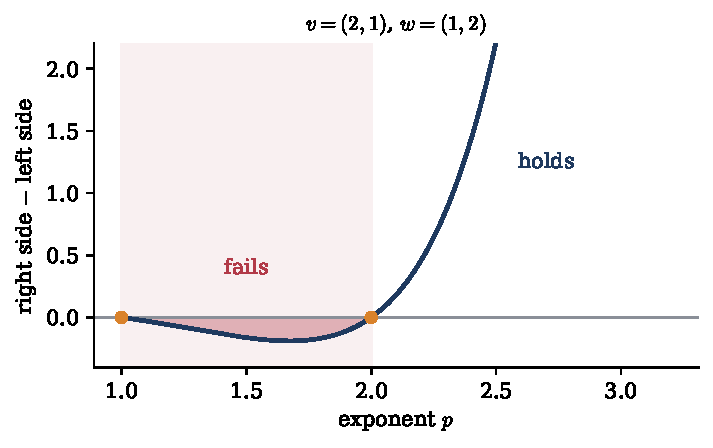
\includegraphics[width=0.62\textwidth]{figures/gap_vs_p.pdf}
\caption{The right side minus the left side of the inequality for $v=(2,1)$ and $w=(1,2)$. It vanishes at $p=1$ and $p=2$, is negative for every $p$ strictly between them, and is positive for every $p>2$. At $p=1.5$ the left side is $3.3431$ and the right side is $3.1803$.}
\label{fig:gap}
\end{figure}

\begin{example}\label{ex:counter}
\consequence\ The pair $v=(2,1)$, $w=(1,2)$ shows that the threshold is sharp in a very simple way. For every $p\in(1,2)$ the inequality fails for this pair, while for $p=1$ and $p=2$ it is an equality (Figure~\ref{fig:gap}). For $p=2$ the pair belongs to the extra equality family of~\cite[Theorem~3]{Paper}, since $v_1w_1=v_2w_2=2$. The same pair, renormalised, gives the counterexamples in Remarks~\ref{rem:fail41} and~\ref{rem:fail21}.
\end{example}

The next two reformulations of~\eqref{eq:loewner} are used repeatedly in the rest of the report. The first evaluates the matrix inequality on a vector, and the second rewrites the theorem in terms of $\ell_p$ norms.

\begin{corollary}[Quadratic form version]\label{cor:quad}
\consequence\ Let $p\ge2$, $v,w\in[0,\infty)^n$ and $s,t\in\R$. Then
\[
\|s\,v^p-t\,w^p\|^2\;\le\;s^2\|v\|^{2p}+t^2\|w\|^{2p}-2st\,\ip vw^p .
\]
In particular $\|v^p-w^p\|^2\le\|v\|^{2p}+\|w\|^{2p}-2\ip vw^p$.
\end{corollary}

\begin{proof}
Evaluate both sides of~\eqref{eq:loewner} on the vector $(s,-t)$.
\end{proof}

\begin{remark}\label{rem:fail21}
\consequence\ For $p=1.5$ and the pair of Example~\ref{ex:counter}, the left side of the special case is $6.6863$ and the right side is $6.3607$. So Corollary~\ref{cor:quad} also needs $p\ge2$.
\end{remark}

For a whole number $p$ the right side of Corollary~\ref{cor:quad} is $\|s\,v^{\otimes p}-t\,w^{\otimes p}\|^2$, where $v^{\otimes p}$ is the $p$-fold tensor power, because $\ip{v^{\otimes p}}{w^{\otimes p}}=\ip vw^p$. The vector $v^p$ is the part of $v^{\otimes p}$ that sits on the diagonal coordinates $(i,i,\dots,i)$, so for whole numbers the corollary says that discarding the off-diagonal coordinates of a tensor power does not increase distances. This is the mechanism behind the proofs in~\cite{JPTV}. For a real exponent there is no tensor power, and Corollary~\ref{cor:quad} is the statement that survives.

\begin{corollary}[Norm version]\label{cor:norms}
\consequence\ Let $p\ge2$ and $v,w\in[0,\infty)^n$, and write $v\circ w$ for the entrywise product. Then
\[
0\;\le\;\ip vw^p-\|v\circ w\|_p^p\;\le\;\|v\|_2^p\|w\|_2^p-\|v\|_{2p}^p\|w\|_{2p}^p .
\]
\end{corollary}

\begin{proof}
Since $\|v^p\|_2=\|v\|_{2p}^p$ and $\ip{v^p}{w^p}=\|v\circ w\|_p^p$, the right inequality is the theorem rearranged. The left one is the superadditivity of $x\mapsto x^p$ applied to $\sum_iv_iw_i$.
\end{proof}

Corollary~\ref{cor:norms} has a plain reading. Passing from $\ell_1$ to $\ell_p$ on the products $v_iw_i$ loses something, and passing from $\ell_2$ to $\ell_{2p}$ on the factors loses something. The theorem says that the first loss never exceeds the second.

\section{Mathematics: entrywise powers and Gram matrices}\label{sec:math}

\paragraph{Many vectors.} \context\ The paper's Proposition~6.1 extends~\eqref{eq:loewner} to $k$ vectors: $\Gram\bigl((v^{(1)})^p,\dots,(v^{(k)})^p\bigr)\preceq\Gram\bigl(v^{(1)},\dots,v^{(k)}\bigr)^{\circ p}$ for $p\in\N\cup[k,\infty)$, and this range cannot be enlarged. The proof uses the theorem of~\cite{GKR15} and is not in Lean.

\paragraph{Eigenvalues and volumes.} \consequence\ Loewner order controls every eigenvalue (Weyl's monotonicity principle) and the determinant. So for $p$ in the range above, the $j$-th largest eigenvalue of the Gram matrix of the powered vectors is at most the $j$-th largest eigenvalue of the entrywise power of the original Gram matrix, and the same holds for the determinants. For two vectors the determinant gives
\[
\|v^p\|^2\|w^p\|^2-\ip{v^p}{w^p}^2\;\le\;\|v\|^{2p}\|w\|^{2p}-\ip vw^{2p}\qquad(p\ge2),
\]
which bounds the squared area of the parallelogram spanned by $v^p$ and $w^p$.

\paragraph{The general pattern.} \context\ FitzGerald and Horn~\cite{FH} found the critical exponent $k-2$ for entrywise powers to preserve positivity of $k\times k$ matrices, and Guillot, Khare and Rajaratnam~\cite{GKR15} found the critical exponents for monotonicity, convexity and superadditivity. Khare's monograph~\cite{Khare} surveys this area. The present result adds a concrete scalar inequality to it whose threshold is exactly a critical exponent. Each monotone functional of Gram matrices turns the matrix theorem into a scalar inequality with the same threshold, so the same method should give sharp thresholds for other inequalities between $\ell_2$ and $\ell_{2p}$ quantities. \proposal\ A systematic search for such functionals, for example ratios of elementary symmetric functions of the eigenvalues, is a natural next step.

\section{Probability: tempered and escort distributions}\label{sec:prob}

This section contains the main application. Let $P$ and $Q$ be probability distributions on a finite set $\{1,\dots,n\}$. Their \emph{Bhattacharyya coefficient}~\cite{Bhattacharyya} is
\[
\BC(P,Q)=\sum_i\sqrt{P_iQ_i}\in[0,1],
\]
and $1-\BC(P,Q)$ is the squared Hellinger distance~\cite{Hellinger} in the normalisation where it lies in $[0,1]$. For $p>0$ the \emph{escort distribution} of order $p$~\cite{BeckSchlogl} is
\[
P^{(p)}_i=\frac{P_i^p}{\sum_jP_j^p}.
\]
\context\ Escort distributions are used in the thermodynamic formalism of multifractals and chaotic systems~\cite{BeckSchlogl}, where $p$ plays the role of an inverse temperature. In statistical physics $P^{(p)}$ is the Gibbs distribution at a temperature $p$ times lower than that of $P$, as made precise in Section~\ref{sec:phys}. In machine learning the same map is called sharpening, as discussed in Section~\ref{sec:ml}. Rényi's entropy of order $p$~\cite{Renyi} is $H_p(P)=\frac1{1-p}\log\sum_iP_i^p$.

\begin{corollary}[Escort distributions]\label{cor:escort}
\consequence\ Let $p\ge2$ and let $P,Q$ be probability distributions on a finite set. Then
\begin{equation}\label{eq:escort}
\sqrt{\textstyle\sum_iP_i^p\,\sum_iQ_i^p}\;\bigl(1-\BC(P^{(p)},Q^{(p)})\bigr)\;\le\;1-\BC(P,Q)^p .
\end{equation}
Equivalently,
\begin{equation}\label{eq:renyi}
1-\BC(P^{(p)},Q^{(p)})\;\le\;e^{\frac{p-1}{2}\,(H_p(P)+H_p(Q))}\,\bigl(1-\BC(P,Q)^p\bigr)\;\le\;p\,e^{\frac{p-1}{2}\,(H_p(P)+H_p(Q))}\,\bigl(1-\BC(P,Q)\bigr).
\end{equation}
For $p>2$ equality holds in~\eqref{eq:escort} only when $P=Q$ or when $P$ and $Q$ are both point masses.
\end{corollary}

\begin{proof}
Apply the theorem to $v=\sqrt P$ and $w=\sqrt Q$, taken entrywise. Then $\|v\|=\|w\|=1$ and $\ip vw=\BC(P,Q)$, so the right side of the theorem is $1-\BC(P,Q)^p$. Also $\|v^p\|^2=\sum_iP_i^p$, and
\[
\ip{v^p}{w^p}=\sum_i(P_iQ_i)^{p/2}=\sqrt{\textstyle\sum_jP_j^p\sum_jQ_j^p}\;\BC(P^{(p)},Q^{(p)}),
\]
so the left side of the theorem is the left side of~\eqref{eq:escort}. The first inequality in~\eqref{eq:renyi} follows because $\sum_iP_i^p=e^{(1-p)H_p(P)}$. The second follows from $1-x^p\le p(1-x)$ for $x\in[0,1]$, which is Bernoulli's inequality. For the equality cases, \cite[Theorem~2]{Paper} says that for $p>2$ equality forces $\sqrt P$ and $\sqrt Q$ to be linearly dependent, which means $P=Q$ because both sum to $1$, or forces each of them to have one nonzero entry.
\end{proof}

\begin{remark}\label{rem:fail41}
\consequence\ The condition $p\ge2$ cannot be relaxed to $p>1$. For $P=(0.8,0.2)$, $Q=(0.2,0.8)$ and $p=1.5$, the left side of~\eqref{eq:escort} is $0.29902$ and the right side is $0.28446$. This is Example~\ref{ex:counter} after normalisation. Figure~\ref{fig:escort} shows that such violations are common for $p=1.5$ and absent for $p=2.5$.
\end{remark}

\begin{figure}[h]
\centering
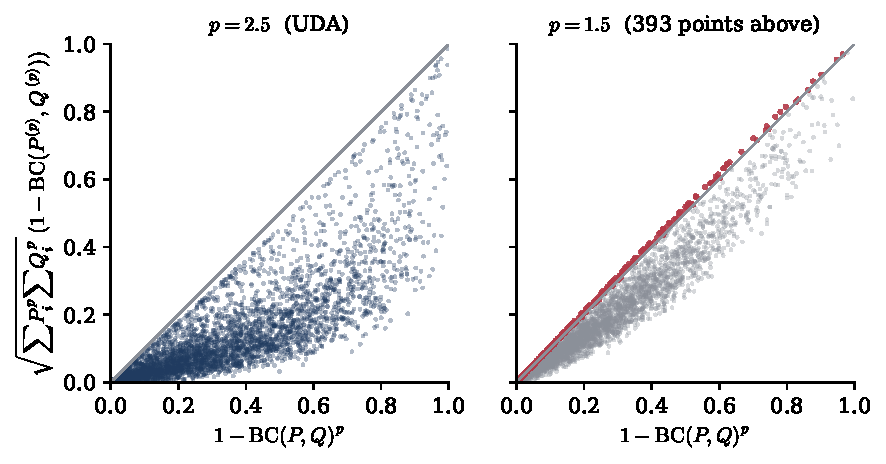
\includegraphics[width=0.92\textwidth]{figures/escort_scatter.pdf}
\caption{Each point is a random pair of distributions on two to five outcomes, plotted with the right side of~\eqref{eq:escort} horizontally and the left side vertically. For $p=2.5$ every point lies below the diagonal, as Corollary~\ref{cor:escort} requires. For $p=1.5$ the red points lie above it.}
\label{fig:escort}
\end{figure}

\paragraph{What the bound says.} Tempering with $p>1$ moves mass towards the most likely outcomes, and two distributions with different modes are pulled apart. The quantity $1-\BC$ measures that separation. Inequality~\eqref{eq:renyi} limits how much tempering can increase it, with a factor that depends only on the Rényi entropies of $P$ and $Q$. When $P$ and $Q$ are already concentrated the factor is close to $1$. Since $H_p\le\log n$ the factor is never more than $n^{p-1}$, so the bound always holds without any condition on the support, but for nearly uniform distributions on many outcomes it is weak.

\paragraph{What it does not say.} \nofollow\ The bound does not show that tempering is contractive, and it does not give a bound that is uniform in the number of outcomes. It also says nothing about softening, which is tempering with $p<1$, because the theorem fails for some pairs when $p<1$~\cite{JPTV}.

\section{Statistical physics: cooling by a factor of at least two}\label{sec:phys}

Consider a system with finitely many states and two energy functions $E$ and $E'$. Let $Z_E(\beta)=\sum_ie^{-\beta E_i}$ be the partition function at inverse temperature $\beta>0$, and let $\bar E=\frac12(E+E')$.

\begin{corollary}[Partition functions]\label{cor:gibbs}
\consequence\ For every $\beta>0$ and every real $p\ge2$,
\[
\sqrt{Z_E(p\beta)\,Z_{E'}(p\beta)}-Z_{\bar E}(p\beta)\;\le\;\bigl(Z_E(\beta)\,Z_{E'}(\beta)\bigr)^{p/2}-Z_{\bar E}(\beta)^p .
\]
If the system has at least two states and $p>2$, equality holds only when $E-E'$ is constant.
\end{corollary}

\begin{proof}
Take $v_i=e^{-\beta E_i/2}$ and $w_i=e^{-\beta E'_i/2}$. Then $\|v\|^2=Z_E(\beta)$, $\ip vw=Z_{\bar E}(\beta)$, $\|v^p\|^2=Z_E(p\beta)$ and $\ip{v^p}{w^p}=Z_{\bar E}(p\beta)$. All entries are positive, so by~\cite[Theorem~2]{Paper} equality for $p>2$ requires $v$ and $w$ to be proportional, which means $E-E'$ is constant.
\end{proof}

\paragraph{Meaning.} By the Cauchy--Schwarz inequality, $Z_{\bar E}(\beta)\le\sqrt{Z_E(\beta)Z_{E'}(\beta)}$, and the ratio of the two sides is the Bhattacharyya coefficient of the Gibbs distributions of $E$ and $E'$ at inverse temperature $\beta$. Corollary~\ref{cor:gibbs} is Corollary~\ref{cor:escort} applied to these Gibbs distributions, and it compares this overlap before and after the system is cooled from inverse temperature $\beta$ to $p\beta$. Figure~\ref{fig:gibbs} shows an example in which cooling by the factor $2.5$ lowers the Bhattacharyya coefficient from $0.897$ to $0.605$.

\begin{figure}[h]
\centering
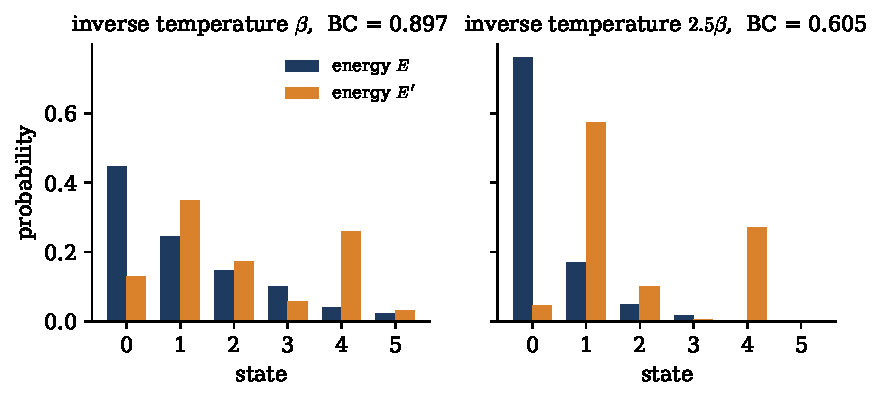
\includegraphics[width=0.92\textwidth]{figures/gibbs_cooling.pdf}
\caption{Gibbs distributions of two energy functions on six states, before and after cooling by the factor $2.5$. Cooling concentrates each distribution on its own ground state, and the overlap falls. Corollary~\ref{cor:gibbs} limits how far it can fall.}
\label{fig:gibbs}
\end{figure}

\paragraph{Degeneracies.} Physical states often come with multiplicities, and coarse-grained models replace them by a density of states $g_i>0$, with $Z_E(\beta;g)=\sum_ig_ie^{-\beta E_i}$. The weighted theorem of the paper~\cite[Theorem~4]{Paper} answers exactly when Corollary~\ref{cor:gibbs} survives this change.

\begin{corollary}[Densities of states]\label{cor:degen}
\consequence\ Let $n\ge2$, $p\ge2$ and $g\in(0,\infty)^n$. The inequality of Corollary~\ref{cor:gibbs}, with every partition function computed with the weights $g$, holds for all energy functions $E,E'$ and all $\beta>0$ if and only if $g_ig_j\ge1$ for all $i\ne j$.
\end{corollary}

\begin{proof}
With the same $v$ and $w$, the weighted partition functions are the weighted norms and inner products of~\cite[Theorem~4]{Paper}, so the condition is sufficient. Conversely, if $g_ig_j<1$, that theorem gives a strict failure at $v=e_i$ and $w=e_j$. Both sides are continuous, so the failure persists for nearby vectors with all entries positive, and every positive vector has the form $(e^{-\beta E_k/2})_k$ for a suitable $E$.
\end{proof}

\begin{figure}[h]
\centering
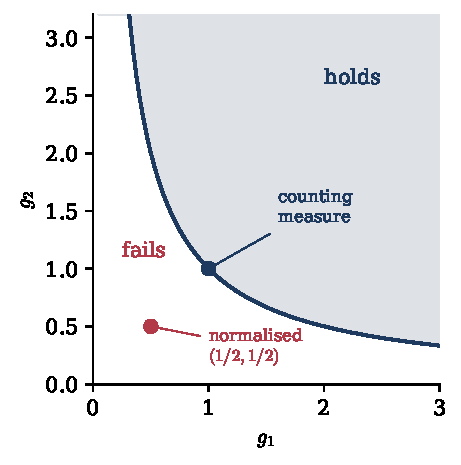
\includegraphics[width=0.36\textwidth]{figures/weights_region.pdf}
\caption{For two states the inequality survives weights $(g_1,g_2)$ exactly in the shaded region $g_1g_2\ge1$. Integer degeneracies always lie in it. A normalised reference measure such as $(1/2,1/2)$ does not.}
\label{fig:weights}
\end{figure}

Integer multiplicities always satisfy the condition, since they amount to repeating states. A reference measure normalised to total mass $1$ on two or more states never does, because then $g_ig_j<1$ for every pair. For example, with $g=(\frac12,\frac12)$, $E=(0,30)$, $E'=(30,0)$, $\beta=1$ and $p=3$, the left side is $0.5000$ and the right side is $0.1250$. The inequality is not homogeneous in $g$, so the scale of the density of states matters. \proposal\ This is a useful warning for anyone who rescales a density of states to a probability measure and expects inequalities between partition functions to persist.

\paragraph{Annealing.} \context\ Simulated annealing~\cite{KGV} and tempering methods move a sampler through a ladder of decreasing temperatures. \proposal\ Corollary~\ref{cor:gibbs} applies to any two rungs whose inverse temperatures differ by a factor of at least $2$, and it bounds how fast two such chains, run with different energy functions, can come apart in Bhattacharyya overlap. Whether this helps the design of temperature ladders is an open question, and the bound says nothing about adjacent rungs closer than a factor of $2$.

\section{Machine learning}\label{sec:ml}

\subsection{Sharpening of predicted distributions}

\context\ Several semi-supervised learning methods sharpen a model's predicted class distribution before using it as a target. MixMatch~\cite{MixMatch} uses $\mathrm{Sharpen}(P,T)_i=P_i^{1/T}/\sum_jP_j^{1/T}$ with $T=0.5$ in all experiments. Unsupervised Data Augmentation~\cite{UDA} divides the logits by a softmax temperature $\tau=0.4$ on its image benchmarks. The Neural Turing Machine~\cite{NTM} sharpens its memory weightings by $w_i\mapsto w_i^\gamma/\sum_jw_j^\gamma$ with a learned $\gamma\ge1$.

All three operations are escort maps. Sharpening with temperature $T$ is the escort of order $p=1/T$. Dividing logits $z$ by $\tau$ gives $\mathrm{softmax}(z/\tau)=\mathrm{softmax}(z)^{(1/\tau)}$, the escort of order $1/\tau$ of the original prediction, because $e^{z_i/\tau}=(e^{z_i})^{1/\tau}$.

\begin{corollary}[Sharpening]\label{cor:sharpen}
\consequence\ Let $P$ and $Q$ be two predicted distributions, for example the predictions for two augmentations of the same input. If they are sharpened with temperature $T\le\frac12$, then with $p=1/T$ inequality~\eqref{eq:escort} bounds the Bhattacharyya affinity of the sharpened predictions in terms of that of the original ones.
\end{corollary}

The three methods fall in different places.
\begin{itemize}
\item MixMatch has $p=2$. This is the case of the original inequality of Johnston and MacLean~\cite{JM19}, and it was already covered before the conjecture was settled.
\item UDA has $p=1/0.4=2.5$. This is a non-integer exponent, and the bound for it needs the new theorem.
\item The Neural Turing Machine allows every $\gamma\ge1$. The bound holds for $\gamma\ge2$, and Remark~\ref{rem:fail41} shows that it can fail for $\gamma$ between $1$ and $2$.
\end{itemize}

\proposal\ Consistency-based methods compare predictions for different augmentations of the same input, and Corollary~\ref{cor:sharpen} says how much sharpening can amplify their disagreement when it is measured by the Bhattacharyya coefficient. This might be used to choose a temperature, or to normalise a consistency loss, but no experiment here tests either use. \nofollow\ Knowledge distillation and calibration by temperature scaling~\cite{Hinton,Guo} usually soften predictions with $T>1$, so $p<1$, and the theorem does not apply there.

\subsection{Kernels on nonnegative features}

Nonnegative feature vectors are common: histograms, word counts, pixel intensities and the outputs of ReLU layers. On such data there are two natural ways to raise a linear kernel to a power $p$:
\[
k_{\mathrm{dot}}(x,y)=\ip xy^p,\qquad k_{\mathrm{pow}}(x,y)=\ip{x^p}{y^p}=\sum_i(x_iy_i)^p .
\]
For whole numbers $p$, $k_{\mathrm{dot}}$ is the homogeneous polynomial kernel~\cite{SchSm}, whose feature map is the tensor power $x\mapsto x^{\otimes p}$, and $k_{\mathrm{pow}}$ keeps only the diagonal part of that feature map. The kernel $k_{\mathrm{pow}}$ is positive semidefinite for every $p>0$, because it has the explicit feature map $x\mapsto x^p$.

\begin{corollary}[Kernel comparison]\label{cor:kernel}
\consequence\ Let $x^{(1)},\dots,x^{(k)}\in[0,\infty)^n$ and let $c\in\R^k$. If $p\in\N\cup[k,\infty)$, then
\[
\sum_{a,b}c_ac_b\,k_{\mathrm{pow}}\bigl(x^{(a)},x^{(b)}\bigr)\;\le\;\sum_{a,b}c_ac_b\,k_{\mathrm{dot}}\bigl(x^{(a)},x^{(b)}\bigr).
\]
For two points and every real $p\ge2$, the distance in the feature space of $k_{\mathrm{pow}}$ satisfies $\|x^p-y^p\|^2\le\|x\|^{2p}+\|y\|^{2p}-2\ip xy^p$.
\end{corollary}

\begin{proof}
The first statement is the $k$-vector Loewner inequality of Section~\ref{sec:math} evaluated on $c$. The second is Corollary~\ref{cor:quad} with $s=t=1$.
\end{proof}

With $c$ equal to $1/m$ on one sample of size $m$ and $-1/m$ on another, the quadratic form in Corollary~\ref{cor:kernel} is the squared maximum mean discrepancy of the two samples~\cite{MMD}. So the discrepancy measured with the diagonal power features never exceeds the one measured with the full polynomial kernel. \nofollow\ For a real exponent the first statement needs $p\ge k$, where $k$ is the number of points, so for real samples of realistic size it only covers whole numbers $p$, and for whole numbers it already follows from the tensor picture. For real $p$ the function $k_{\mathrm{dot}}$ is not even a positive semidefinite kernel on many points unless $p\ge k-2$~\cite{FH}. The two-point statement holds for every real $p\ge2$ and is the part that is new.

\section{Quantum information: where the problem came from}\label{sec:quantum}

\context\ The case $p=2$ was found by Johnston and MacLean~\cite{JM19} while studying pairwise completely positive matrices and quantum states that are invariant under conjugate local diagonal unitaries. Its original proof goes through the separability of a quantum state~\cite[Section~4.1]{JPTV}. For whole numbers $p$, Johnston, Plosker, Torrance and Varona proved the inequality by projecting tensor powers~\cite[Section~3]{JPTV}, which is the picture described after Corollary~\ref{cor:quad}.

\consequence\ For unit vectors $\psi,\phi$ with nonnegative amplitudes and $p\ge2$, the theorem reads
\[
\|\psi^p\|\,\|\phi^p\|-\ip{\psi^p}{\phi^p}\;\le\;1-\ip\psi\phi^p .
\]
When $p$ is a whole number, $\ip\psi\phi^p$ is the overlap of $p$ copies of the two states, and $\psi^p$ is the unnormalised result of projecting $\psi^{\otimes p}$ onto the span of the product states $|i\rangle^{\otimes p}$. \context\ Nonnegative amplitudes are not an exotic assumption. Ground states of stoquastic Hamiltonians can always be chosen nonnegative in the computational basis, by the Perron--Frobenius theorem~\cite{Stoq}.

\nofollow\ For a non-integer $p$ there is no number of copies, and nothing in the theorem gives $\psi^p$ an operational meaning. The real-exponent statement is best read as a fact about the amplitude distributions $|\psi_i|^2$, which brings it back to Section~\ref{sec:prob}.

\section{Limits of the result}\label{sec:limits}

\begin{itemize}
\item \nofollow\ \emph{Exponents below $2$.} The inequality fails for some pairs whenever $0<p<1$ or $1<p<2$~\cite{JPTV}, and every consequence above needs $p\ge2$ or a whole number $p$.
\item \nofollow\ \emph{Vectors with negative entries.} For non-integer $p$ the vector $v^p$ is not defined, and the signed power $(\operatorname{sign}(v_i)|v_i|^p)_i$ raises a different question that is still open~\cite[Section~8]{Paper}.
\item \nofollow\ \emph{Continuous distributions.} All statements here are about finite sums. Extending Corollaries~\ref{cor:escort} and~\ref{cor:gibbs} to densities would need the weighted theorem for general measures, and Corollary~\ref{cor:degen} shows that the normalisation of the measure matters, so the extension is not automatic.
\item \nofollow\ \emph{Sharpness of the constants.} By the equality theorems of~\cite{Paper}, the inequality is strict for $p>2$ outside trivial cases, so the bounds above are attained only by identical distributions or point masses. How much room is left in typical cases is the stability question of~\cite[Section~8]{Paper}.
\end{itemize}

\section{Formal verification as a dependency}

\context\ The theorem, both equality theorems and the weighted characterisation are checked by Lean~4 against Mathlib, using only the three standard axioms~\cite{Repo}. The Loewner inequality~\eqref{eq:loewner} is the Lean lemma \texttt{sum\_psd}. \consequence\ Anyone who builds on the consequences in this report can rely on a machine-checked core, and only the short derivations given here need to be checked by hand. \proposal\ The corollaries of Sections~\ref{sec:core} to~\ref{sec:phys} are a few lines each on top of the existing development and would be easy to add to it.

\section*{Reproducibility}
The script \texttt{consequences.py} tests every corollary on $10^5$ random inputs or more, recomputes every number quoted in this report, and draws the figures. On 8 October 2026 all $19$ checks passed. It needs Python~3 with NumPy and Matplotlib.

\section*{How this report was made}
The author used Claude (Anthropic) to search for consequences of the theorem, to check the cited sources and to draft the text and figures. The author checked the derivations, and each derivation is also tested numerically by the accompanying script.

\appendix
\section{Source audit}\label{app:audit}

\begin{center}
\small
\begin{tabularx}{\textwidth}{@{}p{3.6cm}X@{}}
\toprule
Source & What was checked \\
\midrule
JPTV~\cite{JPTV} & Abstract and Sections 1, 3 and 4.1 of arXiv:2507.10327v1: the integer case, the tensor projection argument (Theorem~3.2) and the separability argument behind the case $p=2$. \\
Johnston--MacLean~\cite{JM19} & Cited through~\cite{JPTV} for the origin of the case $p=2$ in pairwise completely positive matrices. \\
Guillot--Khare--Rajaratnam~\cite{GKR15} & Theorem~5.1 on superadditivity, as used in the paper~\cite{Paper}. \\
MixMatch~\cite{MixMatch} & Equation~(7), the sharpening function, and Section~3.5, which sets $T=0.5$ for all experiments. \\
UDA~\cite{UDA} & Section~2.4 on sharpening by a low softmax temperature, and Appendix~E, which sets $\tau=0.4$ for the CIFAR-10, SVHN and ImageNet experiments. \\
Neural Turing Machine~\cite{NTM} & Equation~(9), the sharpening step with $\gamma_t\ge1$. \\
Bravyi et al.~\cite{Stoq} & The statement that the ground state of a stoquastic Hamiltonian can be chosen as a nonnegative vector, by the Perron--Frobenius theorem. \\
Beck--Schlögl~\cite{BeckSchlogl}, Rényi~\cite{Renyi}, Bhattacharyya~\cite{Bhattacharyya}, Hellinger~\cite{Hellinger} & Standard definitions only. \\
\bottomrule
\end{tabularx}
\end{center}

\begin{thebibliography}{99}\small
\bibitem{BeckSchlogl} C.~Beck and F.~Schlögl, \emph{Thermodynamics of Chaotic Systems: An Introduction}, Cambridge University Press, 1993.
\bibitem{Bhattacharyya} A.~Bhattacharyya, On a measure of divergence between two statistical populations defined by their probability distributions, \emph{Bull. Calcutta Math. Soc.} \textbf{35} (1943), 99--109.
\bibitem{Stoq} S.~Bravyi, D.~P.~DiVincenzo, R.~Oliveira and B.~M.~Terhal, The complexity of stoquastic local Hamiltonian problems, \emph{Quantum Inf. Comput.} \textbf{8} (2008), 361--385. arXiv:quant-ph/0606140.
\bibitem{MixMatch} D.~Berthelot, N.~Carlini, I.~Goodfellow, N.~Papernot, A.~Oliver and C.~Raffel, MixMatch: a holistic approach to semi-supervised learning, \emph{NeurIPS} 2019. arXiv:1905.02249.
\bibitem{FH} C.~H.~FitzGerald and R.~A.~Horn, On fractional Hadamard powers of positive definite matrices, \emph{J. Math. Anal. Appl.} \textbf{61} (1977), 633--642.
\bibitem{Paper} P.~Gaur, A Cauchy--Schwarz inequality for real powers: proof, equality cases and weighted forms, preprint, 2026.
\bibitem{Repo} P.~Gaur, Real-Power-Cauchy-Schwarz, Lean~4 development, 2026. \url{https://github.com/pragyaangaur/Real-Power-Cauchy-Schwarz}.
\bibitem{NTM} A.~Graves, G.~Wayne and I.~Danihelka, Neural Turing machines, arXiv:1410.5401, 2014.
\bibitem{MMD} A.~Gretton, K.~M.~Borgwardt, M.~J.~Rasch, B.~Schölkopf and A.~Smola, A kernel two-sample test, \emph{J. Mach. Learn. Res.} \textbf{13} (2012), 723--773.
\bibitem{GKR15} D.~Guillot, A.~Khare and B.~Rajaratnam, Complete characterization of Hadamard powers preserving Loewner positivity, monotonicity, and convexity, \emph{J. Math. Anal. Appl.} \textbf{425} (2015), 489--507.
\bibitem{Guo} C.~Guo, G.~Pleiss, Y.~Sun and K.~Q.~Weinberger, On calibration of modern neural networks, \emph{ICML} 2017.
\bibitem{Hellinger} E.~Hellinger, Neue Begründung der Theorie quadratischer Formen von unendlichvielen Veränderlichen, \emph{J. Reine Angew. Math.} \textbf{136} (1909), 210--271.
\bibitem{Hinton} G.~Hinton, O.~Vinyals and J.~Dean, Distilling the knowledge in a neural network, arXiv:1503.02531, 2015.
\bibitem{JM19} N.~Johnston and O.~MacLean, Pairwise completely positive matrices and conjugate local diagonal unitary invariant quantum states, \emph{Electron. J. Linear Algebra} \textbf{35} (2019), 156--180.
\bibitem{JPTV} N.~Johnston, S.~Plosker, C.~Torrance and L.~M.~B.~Varona, Generalizing the Cauchy--Schwarz inequality: Hadamard powers and tensor products, \emph{Linear Multilinear Algebra} (2026), doi:10.1080/03081087.2026.2707240. arXiv:2507.10327.
\bibitem{Khare} A.~Khare, \emph{Matrix Analysis and Entrywise Positivity Preservers}, London Math. Soc. Lecture Note Ser. 471, Cambridge University Press, 2022.
\bibitem{KGV} S.~Kirkpatrick, C.~D.~Gelatt and M.~P.~Vecchi, Optimization by simulated annealing, \emph{Science} \textbf{220} (1983), 671--680.
\bibitem{Renyi} A.~Rényi, On measures of entropy and information, \emph{Proc. Fourth Berkeley Symp. Math. Statist. Probab.} \textbf{1} (1961), 547--561.
\bibitem{SchSm} B.~Schölkopf and A.~J.~Smola, \emph{Learning with Kernels}, MIT Press, 2002.
\bibitem{UDA} Q.~Xie, Z.~Dai, E.~Hovy, M.-T.~Luong and Q.~V.~Le, Unsupervised data augmentation for consistency training, \emph{NeurIPS} 2020. arXiv:1904.12848.
\end{thebibliography}

\end{document}
